%%%%%%%%%%%%%%%%%%%%%%%%%%%%%%%%%%%%%%%%%%%%%%%%%%%%%%%%%%%%%%%%%%%%%%%%%%%%%%%%%%%%%
\clearpage
\section{Structure factors for Yukawa like potentials}~\\
\label{sect:SQ4Yukawa}
For charged colloidal dispersions analytical structure factors have been found in the mean spherical approximation \cite{Hayter1981,Hansen1982,Liu2005}. The hard core Yukawa potential (also called a screened Coulomb potential) is defined as
\begin{align}
u^\mathrm{Y}(r,K,Z) &= k_BT \begin{cases}
                             \infty, & \mbox{if } 0\leq r < \sigma \\
                             -\frac{K}{r/\sigma}\exp(-Z (r/\sigma-1)), & r\leq \sigma.
                            \end{cases}
\end{align}
In the limit of no screening, i.e. $Z=0$ the interaction is a purely Coloumb interaction proportional to $1/r$.

\subsection{Hard core double Yukawa interaction}~\\
\label{sect:SQ4doubleYukawa}
To describe a short range attractive and long range repulsive interaction Liu et al.\ \cite{Liu2005} calculated an analytical solution of Ornstein-Zernike equation in the mean spherical approximation. They assumed a potential of the form
\begin{align}\label{eq:SQ2Ypotential}
\frac{u^\mathrm{2Y}(r,\ldots)}{k_BT} &= \begin{cases}
                             \infty, & \mbox{if }  r < \sigma \\
                             -K_1\frac{\exp\left(-Z_1 \left(\frac{r}{\sigma}-1\right)\right)}{r/\sigma} -K_2\frac{\exp\left(-Z_2 \left(\frac{r}{\sigma}-1\right)\right)}{r/\sigma}, & r\leq \sigma.
                            \end{cases}
\end{align}
\begin{figure}[htb]
\begin{center}
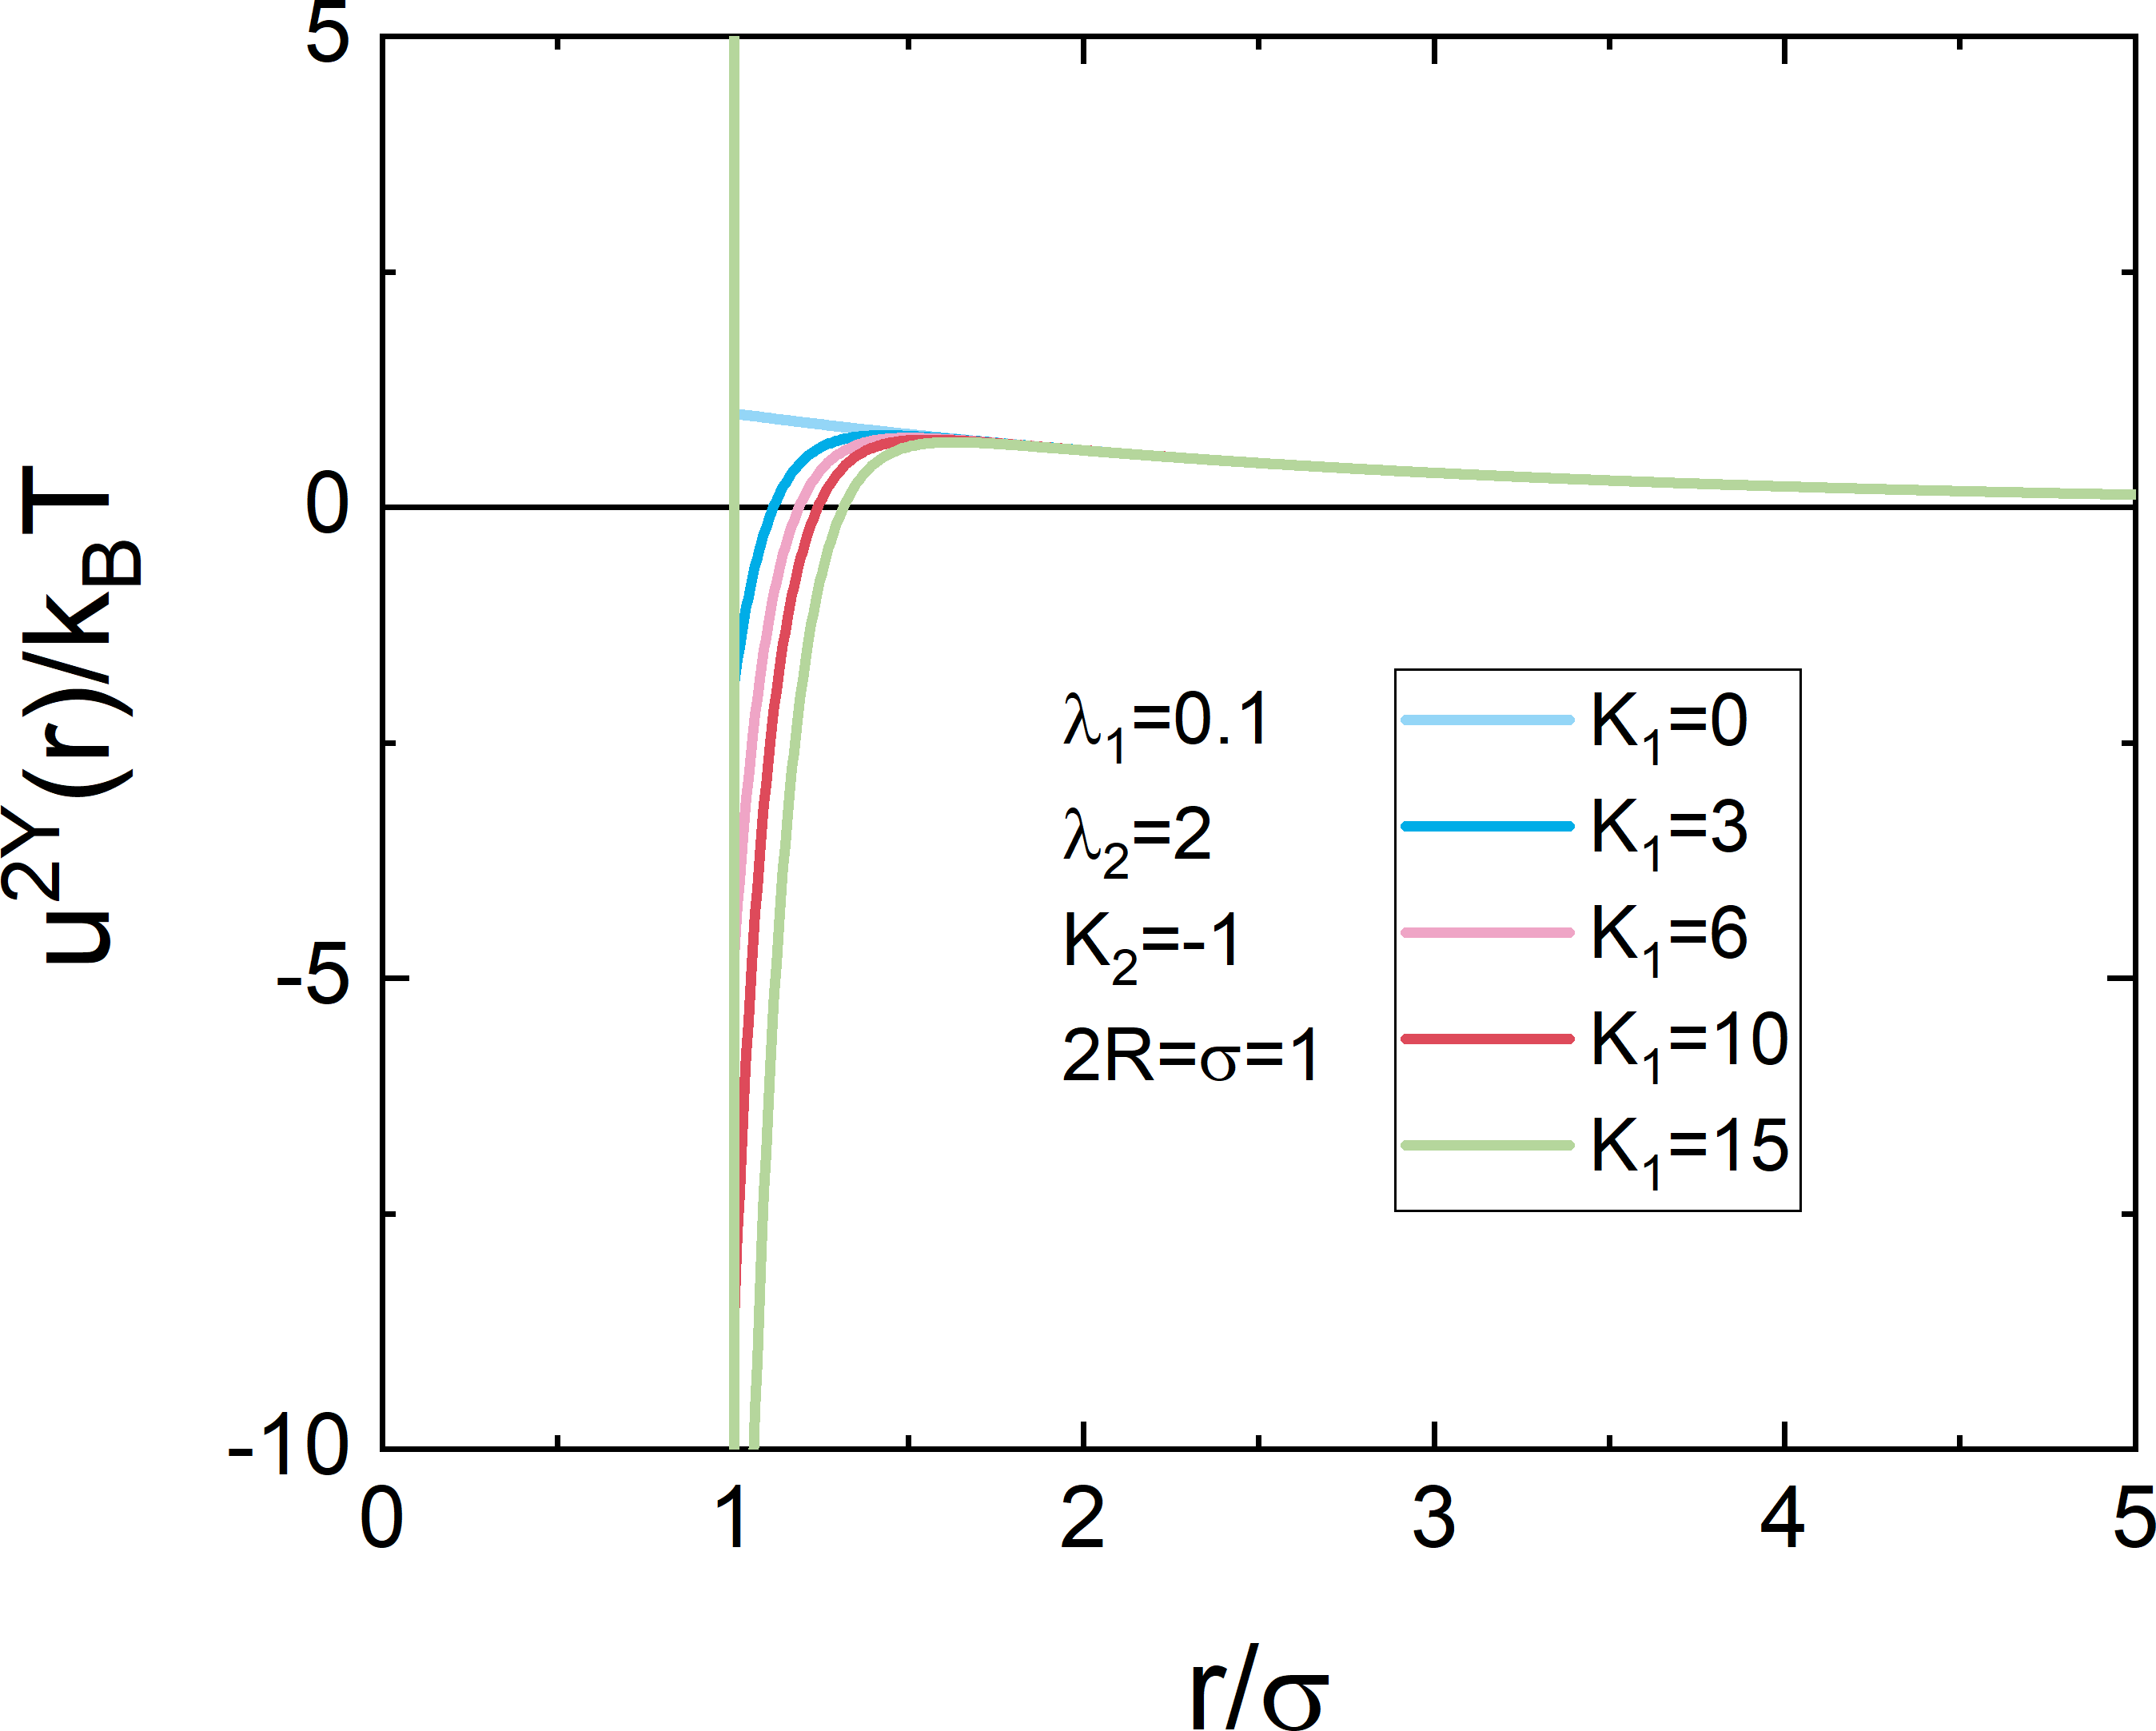
\includegraphics[width=0.768\textwidth]{../images/structure_factor/YukawaLike/TwoYukawaPotential.png}
\end{center}
\caption{potential two-Yukawa potential.} \label{fig:2YukawaPotential}
\end{figure}

\begin{figure}[htb]
\begin{center}
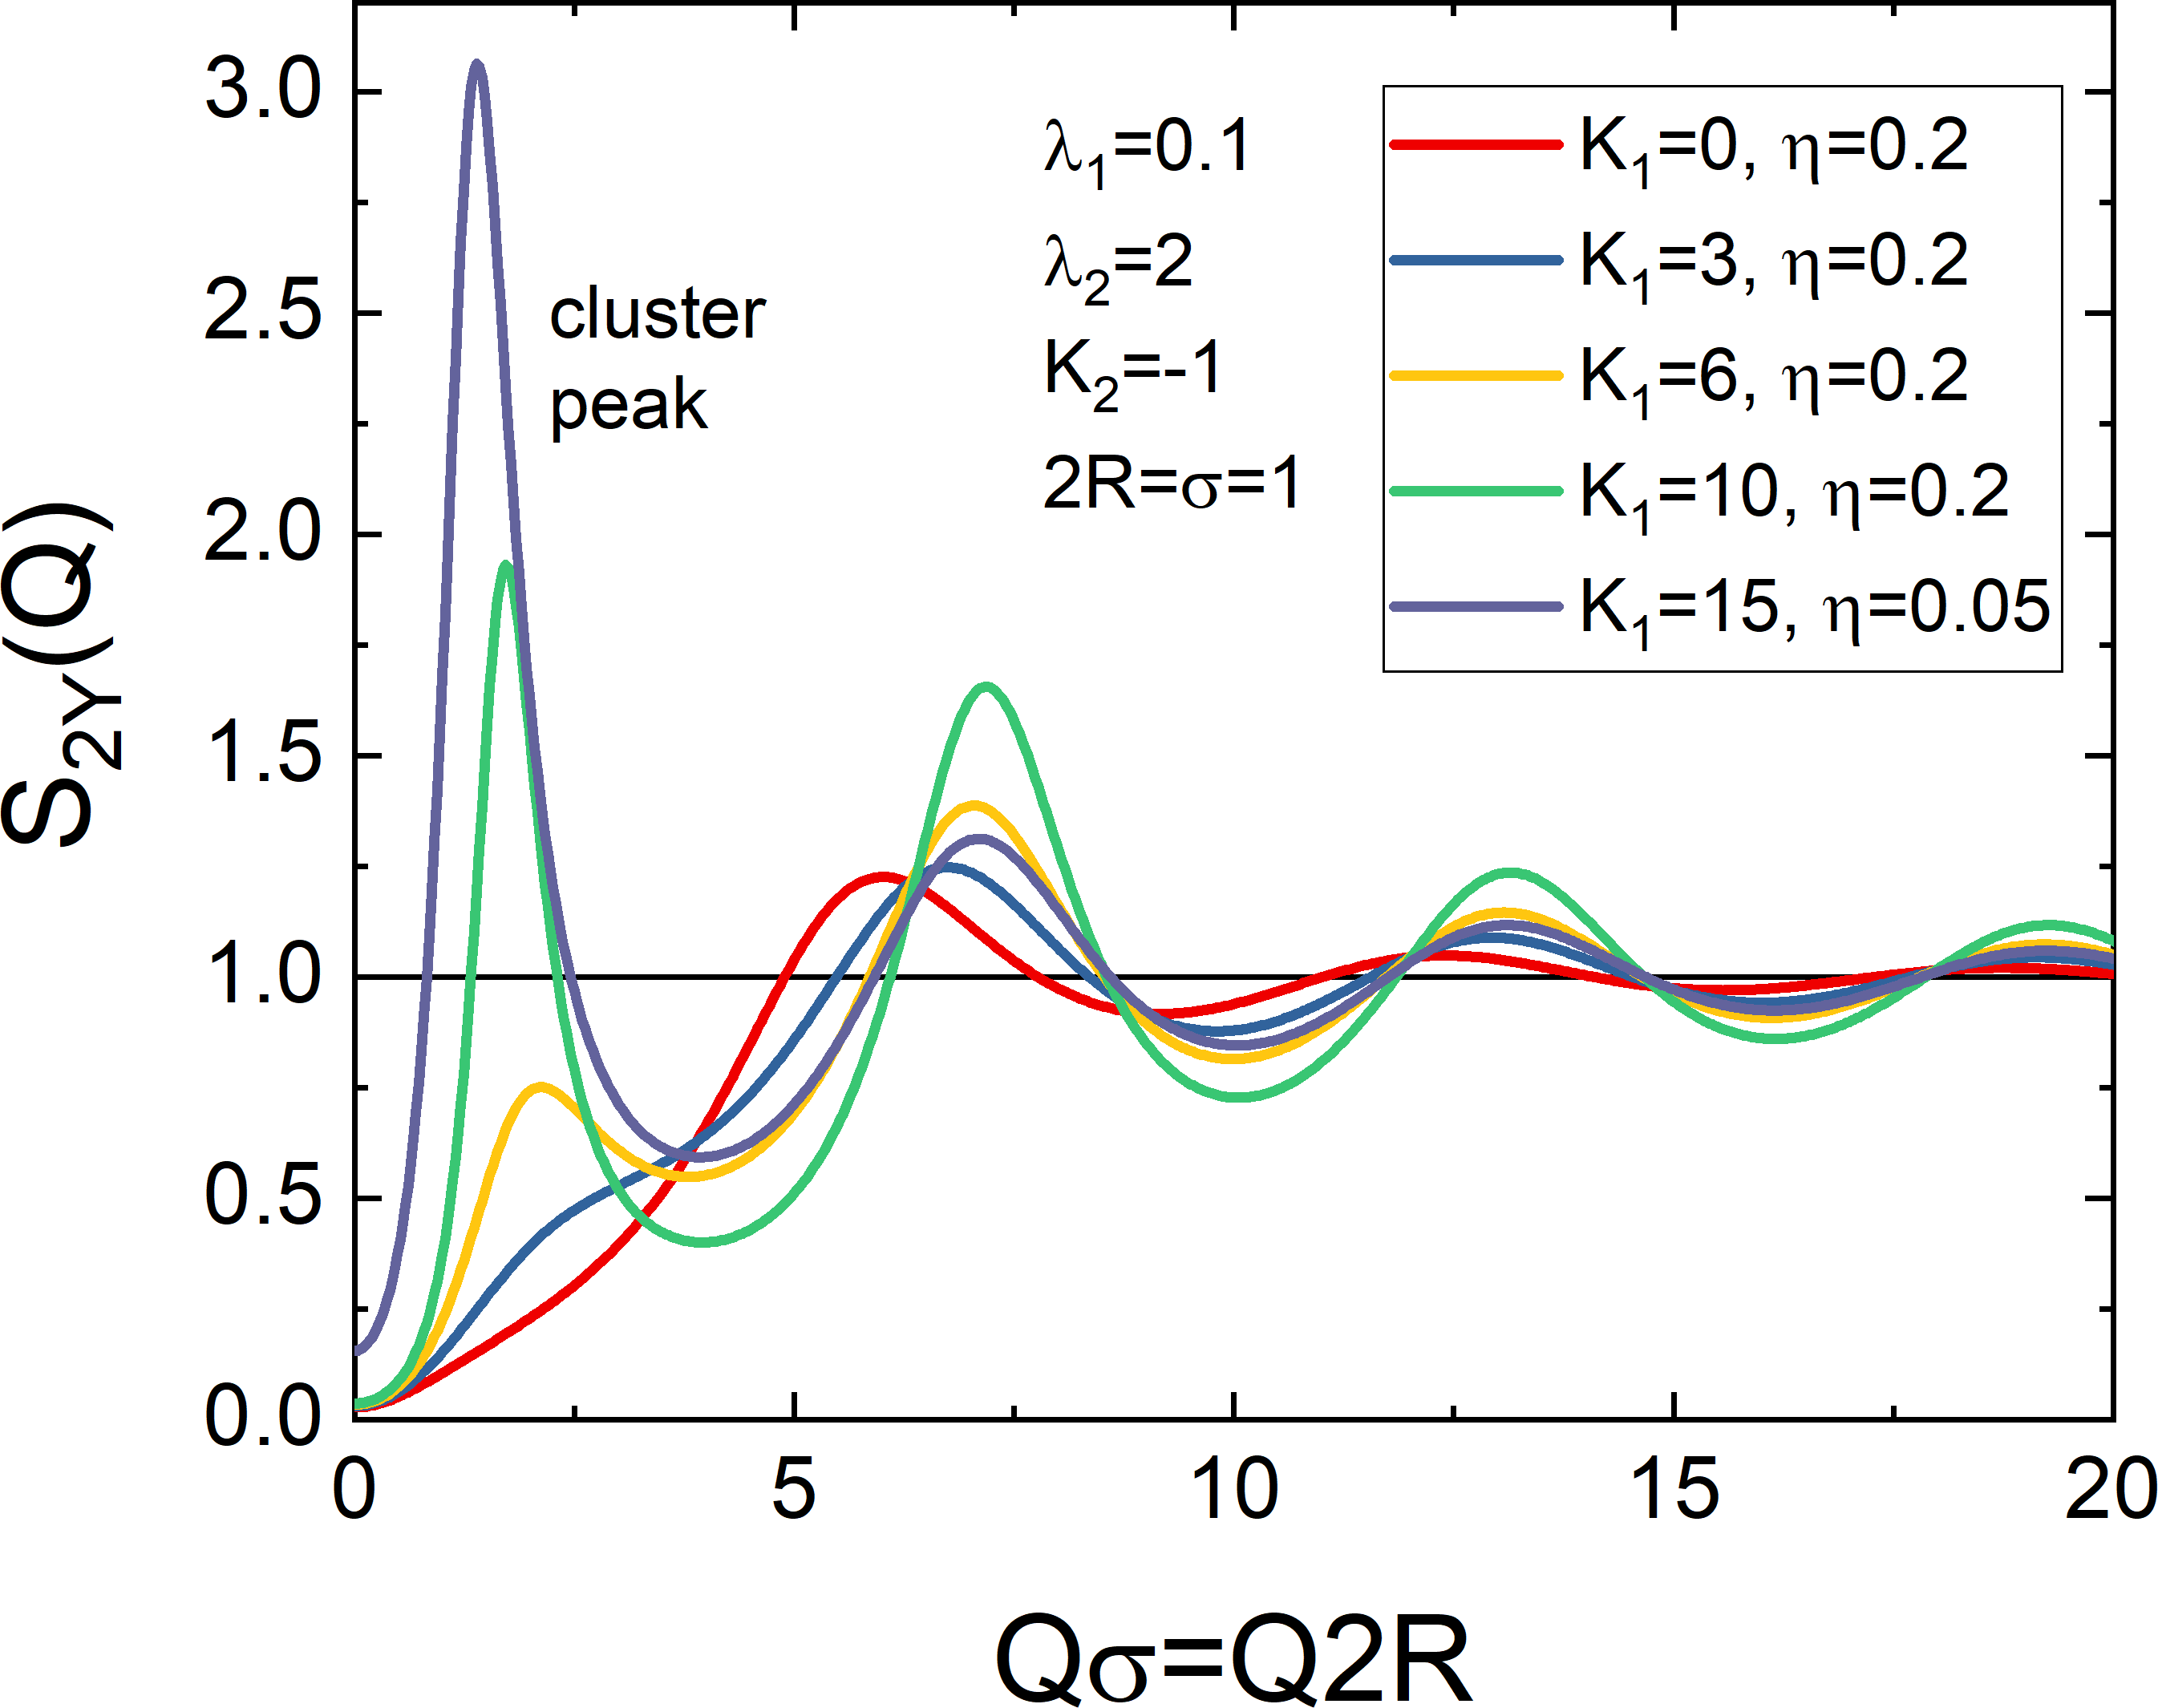
\includegraphics[width=0.768\textwidth]{../images/structure_factor/YukawaLike/TwoYukawa.png}
\end{center}
\caption{Structure factor of two-Yukawa potential in the mean spherical approximation showing a cluster peak.} \label{fig:2Yukawa}
\end{figure}

\noindent\underline{Note:}
\begin{itemize}
  \item The code in \SASfit is based on Matlab code supplied by Yun Liu. The XOP version of this function is based in parts on c-code supplied by Marcus Henning and used for the implementation of this plugin.
  \item For nonphysical or no solution an error message is returned.
  \item For values close to $Z_1=Z_2$ the separately implemented structure factor a single Yukawa interaction potential should be used.
\end{itemize} 